\documentclass[a4paper,12pt]{report}
\usepackage{color}
\usepackage{hyperref}
\hypersetup{
    colorlinks,
    citecolor=black,
    filecolor=black,
    linkcolor=black,
    urlcolor=black
}
\setcounter{secnumdepth}{0}
\usepackage{graphicx}
\usepackage{epstopdf}
\epstopdfsetup{outdir=./}
\usepackage{amsmath}
\usepackage[table,xcdraw]{xcolor}
\usepackage{amssymb}
\usepackage{listings}
\definecolor{anti-flashwhite}{rgb}{0.95, 0.95, 0.96}
\lstset{
	language=C++,
    basicstyle=\ttfamily,
    keywordstyle=\color{blue}\ttfamily,
    stringstyle=\color{red}\ttfamily,
	commentstyle=\color{green}\ttfamily,
    morecomment=[l][\color{magenta}]{\#},
    backgroundcolor=\color{anti-flashwhite}
}
\begin{document}
\title{
\textbf{Distributed Computing - II: CS5320}\\~\\
\begin{huge}
\textbf{Programming Assignment 2:\\Termination Detection
\\~\\}
\end{huge}
\begin{huge}
\textbf{Assignment Report}
\end{huge}
}
\author{\textbf{Sagar Jain - CS17BTECH11034}\\}
\maketitle
\begin{large}
\tableofcontents
\end{large}
\newpage
\section{Program Design}
\subsection{Spanning Tree Algorithm}
\subsubsection{Cell Struct}
The cell struct represents each node in the distributed network. The following constitutes the cell.
\begin{enumerate}
\item A vector of all the children nodes of the node i.e. \textbf{children}.
\item A boolean array which represents if the tokens were received from a particular node i.e \textbf{tokenReceived}.
\item A boolean which represents if a node has a token or not i.e. \textbf{haveToken}.
\item \textbf{cellColour}, the colour of the cell.
\item \textbf{nodeColour}, the colout of the node, which also ends up becoming the colour of the token which the node sends to its parent.
\item A mutex lock which is used to achieve mutual exclusion every time data of this cell is being accessed i.e \textbf{lock}.
\end{enumerate}
\subsubsection{Cell Process}
This is the function which every cell runs when it is launched, it also launches another process which is used to receive messages from other threads. The following are the main tasks of this function.
\begin{enumerate}
\item Launch the receiving threads.
\item Wait for the listening threads to begin listening before beginning to send messages. This is done using \textbf{pthread\_cond\_wait}.
\item Start sending encoded messages of the colour of the cell (red or blue) to a corresponding number of the neighbours of the cell.
\item After each round of sending messages, check if the cell has received tokens from all the children and if so, if the cell itself is currently blue, if both theses condition are satisfied then send a token of the colour of the node (\textbf{node colour and cell colour are different things}) to the parent.
\item Once a token is sent to the parent, the \textbf{receivedToken} vector has all its entries sent to false as we must wait for all the childrent to send tokens once again before this cell can send a token to its parent,
\end{enumerate}
\subsubsection{Receiver Process}
This function is responsible for handling the receiving of messages from other cells, and taking appropriate action on the receipt of said messages.
The main tasks of this function are highlighted below:
\begin{enumerate}
\item The receiving process first sets up the listening server, and after each server is set up it increments a variable in the critical section, using  a \textbf{pthread\_conditional\_variable} we can broadcast to all the sending threads that they can begin sending messages once the value of this variable is equal to the number of cells.
\item On receiving a message the receiving thread decodes the contents of the message, i.e. the sender id and the encoded digit which signifies the colour of the node cell or the colour of the token. A message can either be one which contains a token or one which contains the colour of the sender.
\item After decoding the contents of the message a given cell, changes or doesn't change its cell colour and/or node colour based on the contents of the received message.
\end{enumerate}
\subsubsection{Miscellaneous}
The following is the message encoding format and meaning:\\
Every message begins with the sender id, this is followed by a delimiting \#, that is followed by one of the following numbers,\\
 1 - White Cell\\
 2 - Red Cell\\
 3 - Blue Cell\\
 4 - White Token\\
 5 - Black Token\\
\subsection{Message Optimal Algorithm}
\newpage
\section{Program Output}
\subsection{Spanning Tree Algorithm}
\subsection{Message Optimal Algorithm}
\newpage
\section{Results \& Graphs}
\subsection{Spanning Tree Algorithm}
\begin{center}
\begin{large}
\textbf{Number of Processes Vs Number of Control Message}\\
\end{large}
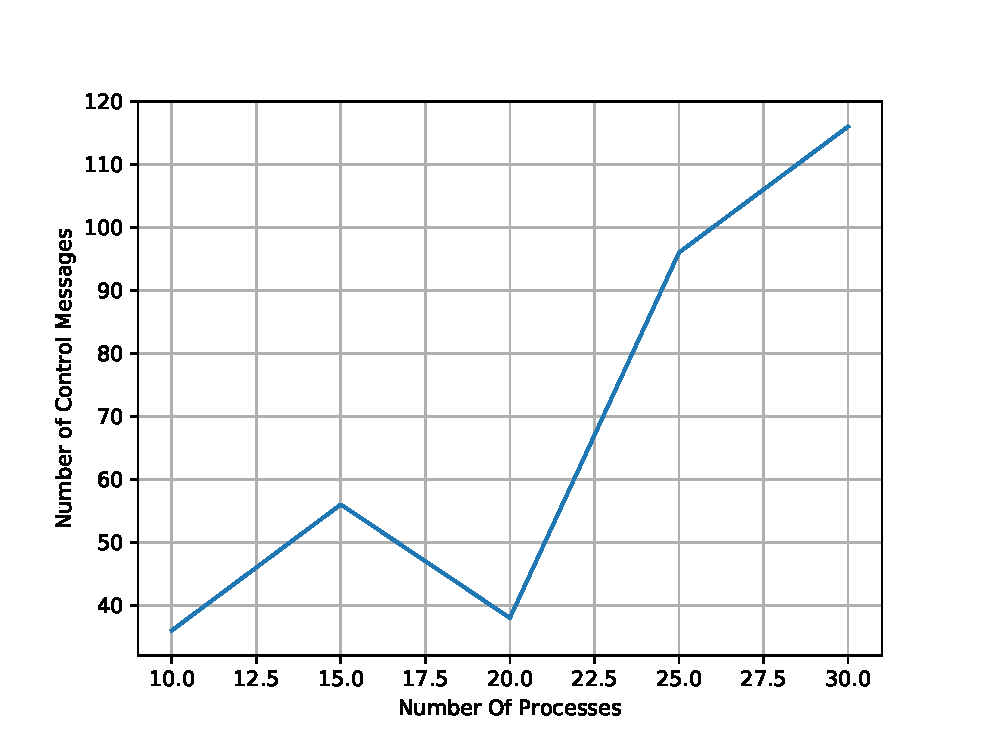
\includegraphics[scale=0.7]{./ncm.eps}
\end{center}
\begin{center}
\begin{large}
\textbf{Number of Processes Vs Time Taken}\\
\end{large}
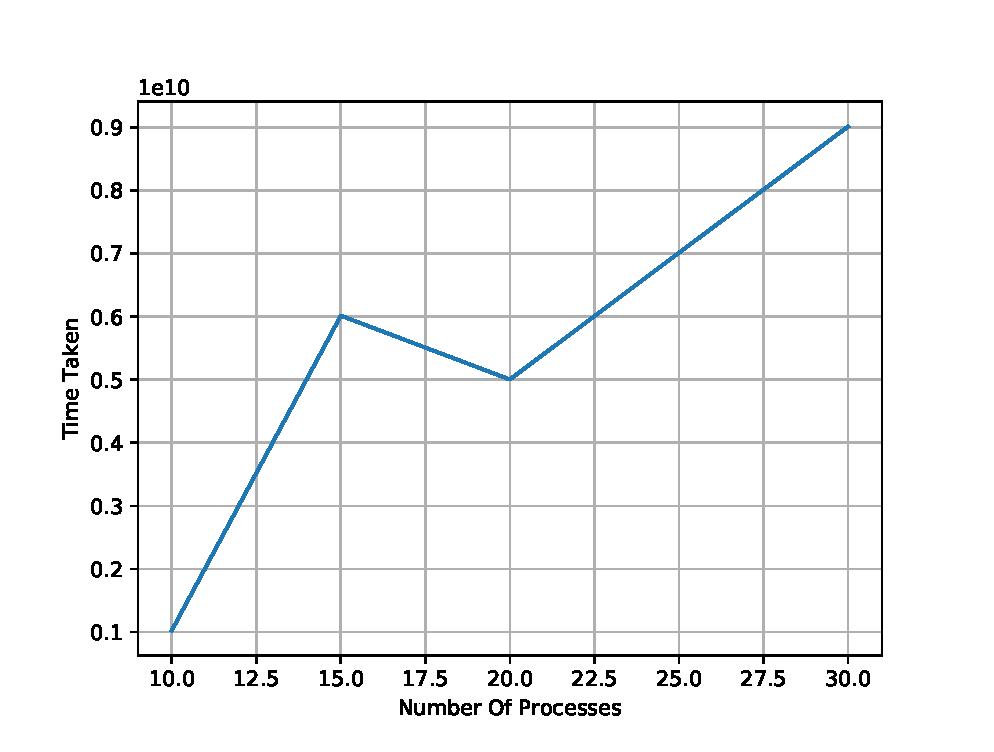
\includegraphics[scale=0.7]{./tt.eps}
\end{center}
\subsection{Explaination of Results}
The following are a few points to note / observations about the above graphs:
\begin{enumerate}
\item
\end{enumerate}
\newpage
\subsection{Message Optimal Algorithm}
\begin{center}
\begin{large}
\textbf{G1}\\
\end{large}
%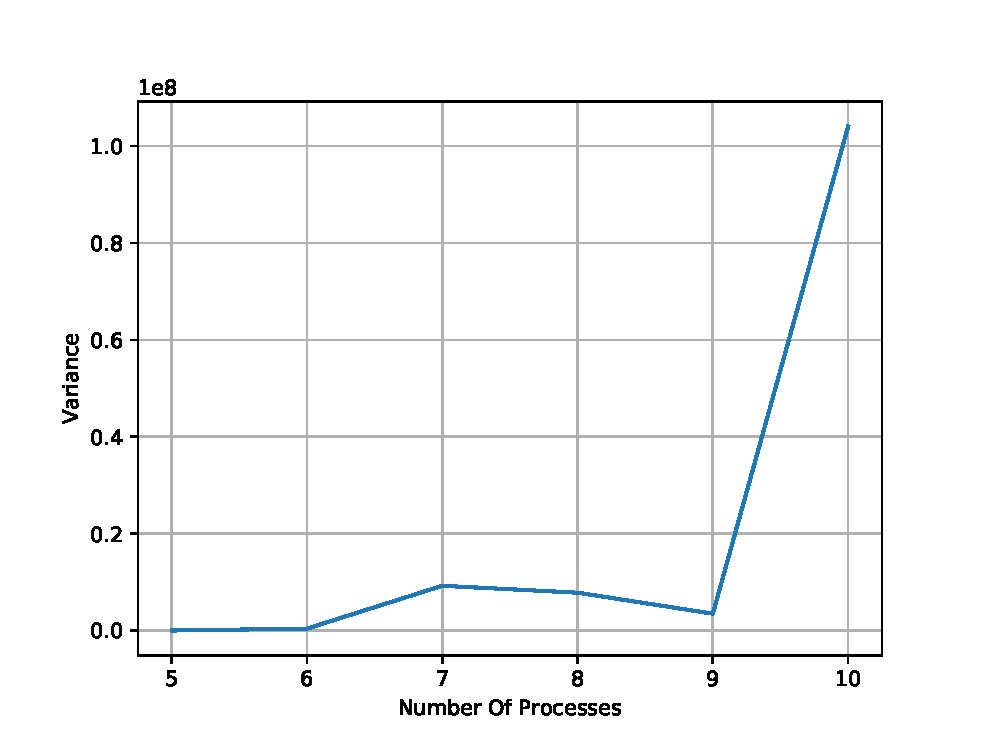
\includegraphics[scale=0.7]{./constantK.eps}
\end{center}
\begin{center}
\begin{large}
\textbf{G2}\\
\end{large}
%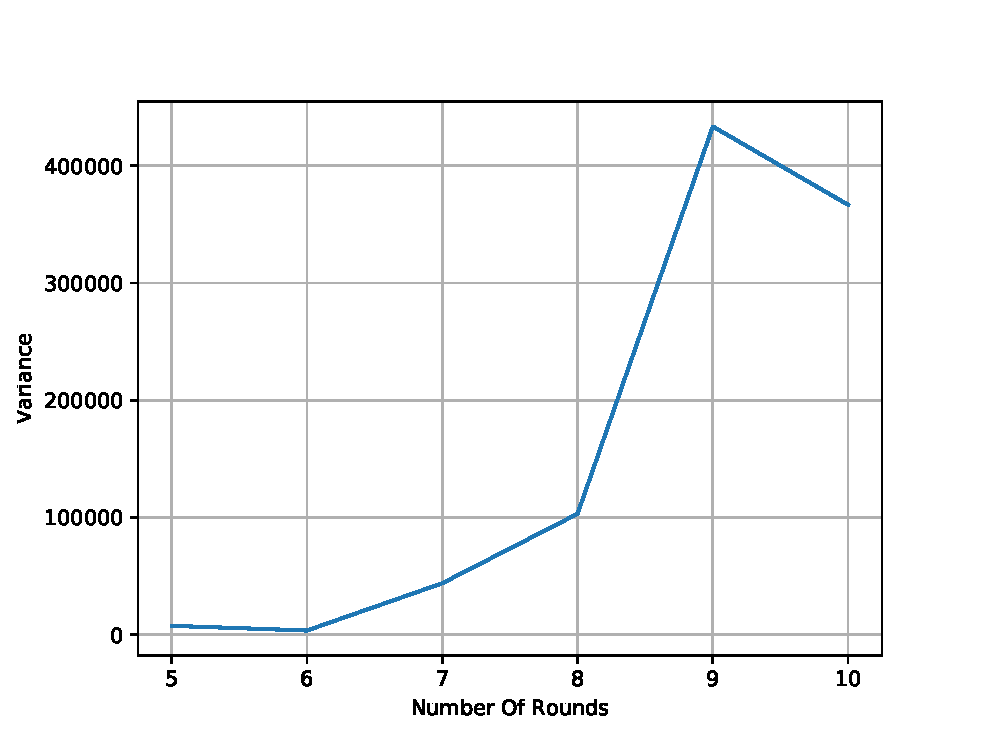
\includegraphics[scale=0.7]{./constantN.eps}
\end{center}
\subsection{Explaination of Results}
The following are a few points to note / observations about the above graphs:
\begin{enumerate}
\item
\end{enumerate}
\end{document}